\section{XMText  Class Reference}
\label{classXMText}\index{XMText@{XMText}}
{\tt \#include $<$XMText.h$>$}

Inheritance diagram for XMText::\begin{figure}[H]
\begin{center}
\leavevmode
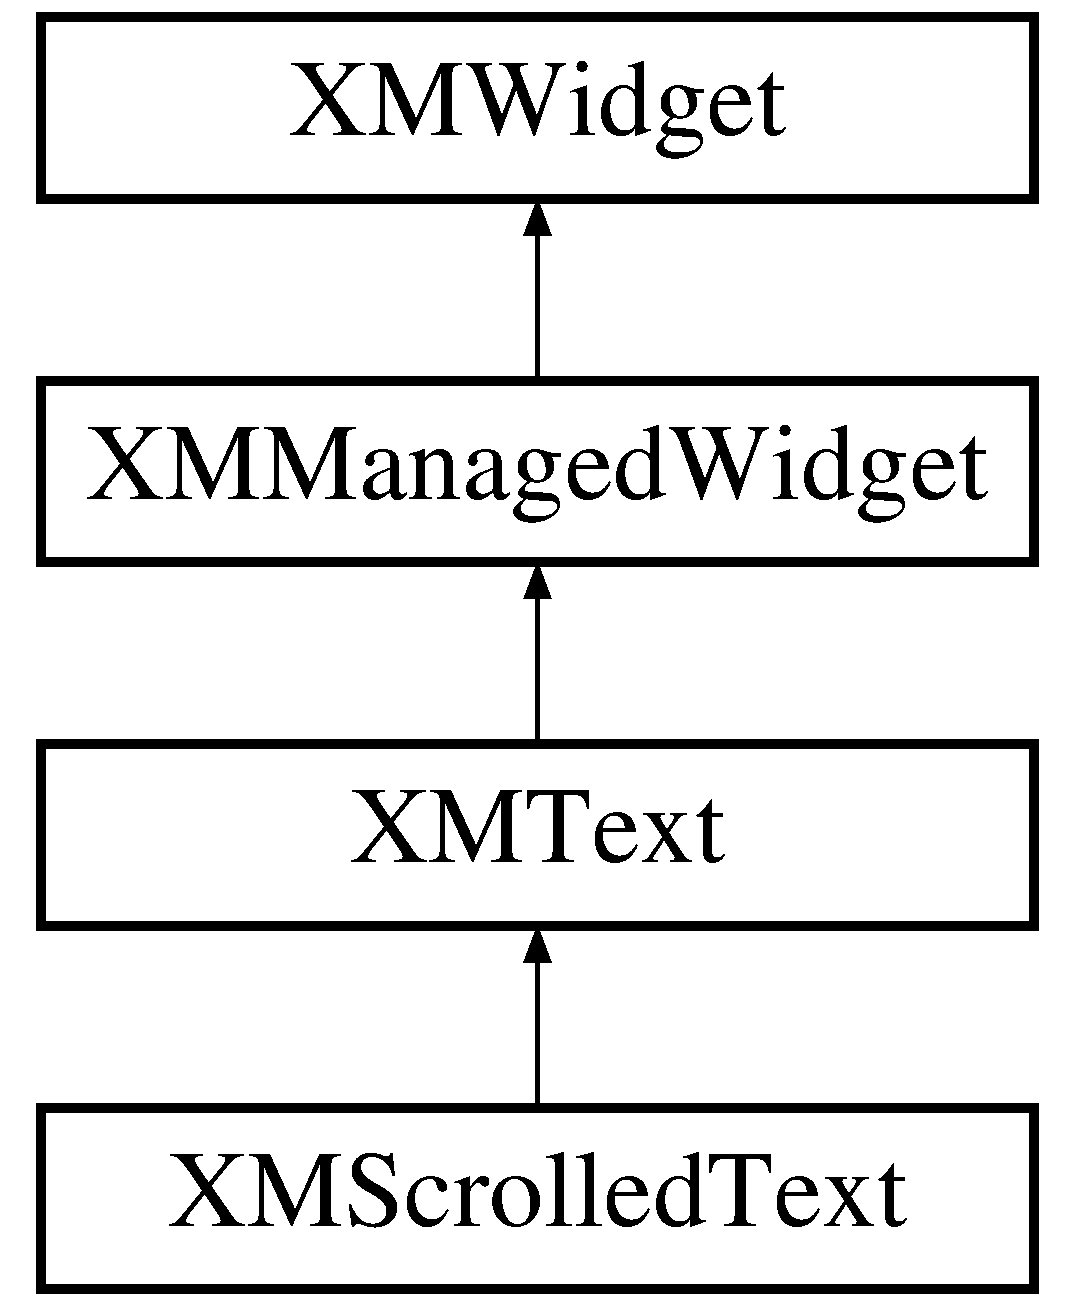
\includegraphics[height=4cm]{classXMText}
\end{center}
\end{figure}
\subsection*{Public Methods}
\begin{CompactItemize}
\item 
{\bf XMText} (char $\ast$n, {\bf XMWidget} \&parent, int rows=1, int columns=30, Arg\-List args=NULL, Cardinal arg\_\-count=0)
\item 
{\bf XMText} (char $\ast$n, Widget parent, int rows=1, int columns=30, Arg\-List args=NULL, Cardinal arg\_\-count=0)
\item 
{\bf XMText} (char $\ast$n)
\item 
{\bf XMText} (Widget w)
\item 
void {\bf Set\-Columns} (int columns)
\item 
void {\bf Set\-Rows} (int rows)
\item 
void {\bf Set\-Max\-Length} (int len)
\item 
void {\bf Enable\-Word\-Wrap} ()
\item 
void {\bf Disable\-Word\-Wrap} ()
\item 
char $\ast$ {\bf Get\-Text} ()
\item 
void {\bf Set\-Text} (char $\ast$txt)
\item 
void {\bf Set\-Editing} (Boolean enable)
\end{CompactItemize}


\subsection{Constructor \& Destructor Documentation}
\index{XMText@{XMText}!XMText@{XMText}}
\index{XMText@{XMText}!XMText@{XMText}}
\subsubsection{\setlength{\rightskip}{0pt plus 5cm}XMText::XMText (char $\ast$ {\em n}, {\bf XMWidget} \& {\em parent}, int {\em rows} = 1, int {\em columns} = 30, Arg\-List {\em args} = NULL, Cardinal {\em arg\_\-count} = 0)\hspace{0.3cm}{\tt  [inline]}}\label{classXMText_a0}




Definition at line 305 of file XMText.h.

References Set\-Columns(), and Set\-Rows().\index{XMText@{XMText}!XMText@{XMText}}
\index{XMText@{XMText}!XMText@{XMText}}
\subsubsection{\setlength{\rightskip}{0pt plus 5cm}XMText::XMText (char $\ast$ {\em n}, Widget {\em parent}, int {\em rows} = 1, int {\em columns} = 30, Arg\-List {\em args} = NULL, Cardinal {\em arg\_\-count} = 0)\hspace{0.3cm}{\tt  [inline]}}\label{classXMText_a1}




Definition at line 312 of file XMText.h.

References Set\-Columns(), and Set\-Rows().\index{XMText@{XMText}!XMText@{XMText}}
\index{XMText@{XMText}!XMText@{XMText}}
\subsubsection{\setlength{\rightskip}{0pt plus 5cm}XMText::XMText (char $\ast$ {\em n})\hspace{0.3cm}{\tt  [inline]}}\label{classXMText_a2}




Definition at line 319 of file XMText.h.\index{XMText@{XMText}!XMText@{XMText}}
\index{XMText@{XMText}!XMText@{XMText}}
\subsubsection{\setlength{\rightskip}{0pt plus 5cm}XMText::XMText (Widget {\em w})\hspace{0.3cm}{\tt  [inline]}}\label{classXMText_a3}




Definition at line 320 of file XMText.h.

\subsection{Member Function Documentation}
\index{XMText@{XMText}!DisableWordWrap@{DisableWordWrap}}
\index{DisableWordWrap@{DisableWordWrap}!XMText@{XMText}}
\subsubsection{\setlength{\rightskip}{0pt plus 5cm}void XMText::Disable\-Word\-Wrap ()\hspace{0.3cm}{\tt  [inline]}}\label{classXMText_a8}




Definition at line 336 of file XMText.h.

References XMWidget::Set\-Attribute().\index{XMText@{XMText}!EnableWordWrap@{EnableWordWrap}}
\index{EnableWordWrap@{EnableWordWrap}!XMText@{XMText}}
\subsubsection{\setlength{\rightskip}{0pt plus 5cm}void XMText::Enable\-Word\-Wrap ()\hspace{0.3cm}{\tt  [inline]}}\label{classXMText_a7}




Definition at line 333 of file XMText.h.

References XMWidget::Set\-Attribute().\index{XMText@{XMText}!GetText@{GetText}}
\index{GetText@{GetText}!XMText@{XMText}}
\subsubsection{\setlength{\rightskip}{0pt plus 5cm}char$\ast$ XMText::Get\-Text ()\hspace{0.3cm}{\tt  [inline]}}\label{classXMText_a9}




Definition at line 339 of file XMText.h.

References XMWidget::id.\index{XMText@{XMText}!SetColumns@{SetColumns}}
\index{SetColumns@{SetColumns}!XMText@{XMText}}
\subsubsection{\setlength{\rightskip}{0pt plus 5cm}void XMText::Set\-Columns (int {\em columns})\hspace{0.3cm}{\tt  [inline]}}\label{classXMText_a4}




Definition at line 324 of file XMText.h.

References XMWidget::Set\-Attribute().

Referenced by XMScrolled\-Text::XMScrolled\-Text(), and XMText().\index{XMText@{XMText}!SetEditing@{SetEditing}}
\index{SetEditing@{SetEditing}!XMText@{XMText}}
\subsubsection{\setlength{\rightskip}{0pt plus 5cm}void XMText::Set\-Editing (Boolean {\em enable})\hspace{0.3cm}{\tt  [inline]}}\label{classXMText_a11}




Definition at line 344 of file XMText.h.

References XMWidget::Set\-Attribute().\index{XMText@{XMText}!SetMaxLength@{SetMaxLength}}
\index{SetMaxLength@{SetMaxLength}!XMText@{XMText}}
\subsubsection{\setlength{\rightskip}{0pt plus 5cm}void XMText::Set\-Max\-Length (int {\em len})\hspace{0.3cm}{\tt  [inline]}}\label{classXMText_a6}




Reimplemented in {\bf XMScrolled\-Text} {\rm (p.\,\pageref{classXMScrolledText_a2})}.

Definition at line 330 of file XMText.h.

References XMWidget::Set\-Attribute().\index{XMText@{XMText}!SetRows@{SetRows}}
\index{SetRows@{SetRows}!XMText@{XMText}}
\subsubsection{\setlength{\rightskip}{0pt plus 5cm}void XMText::Set\-Rows (int {\em rows})\hspace{0.3cm}{\tt  [inline]}}\label{classXMText_a5}




Definition at line 327 of file XMText.h.

References XMWidget::Set\-Attribute().

Referenced by XMScrolled\-Text::XMScrolled\-Text(), and XMText().\index{XMText@{XMText}!SetText@{SetText}}
\index{SetText@{SetText}!XMText@{XMText}}
\subsubsection{\setlength{\rightskip}{0pt plus 5cm}void XMText::Set\-Text (char $\ast$ {\em txt})\hspace{0.3cm}{\tt  [inline]}}\label{classXMText_a10}




Definition at line 341 of file XMText.h.

References XMWidget::id.

The documentation for this class was generated from the following file:\begin{CompactItemize}
\item 
{\bf XMText.h}\end{CompactItemize}
